\section{Priority Based Consistent Hashing} % Based Load Balancing Policies}
\label{sec:qos-chrlu}

In this section, we extend the load-balancing algorithm to take into consideration function \emph{priority}, in addition to the characteristics in Section~\ref{sec:chrlu}. 
% We assume a cluster of homogeneous servers, and that a new function invocation can be sent to any of the servers.
% Each server implements keep-alive for functions: after successful execution, the function's container is stored in server memory, and evicted based on some eviction policy.

\begin{figure}
\centering
  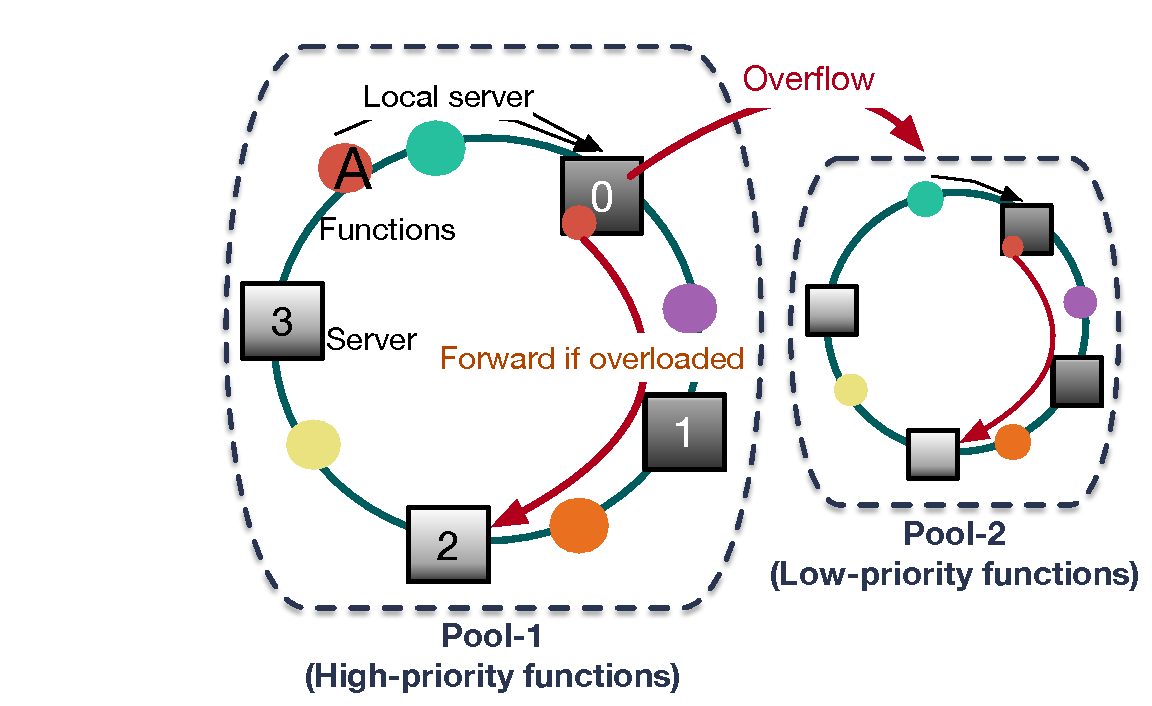
\includegraphics[width=0.8\textwidth]{chrlu/qos/figs/k-rlu2.pdf}
  \caption{$k$-CH-RLU partitions a cluster into multiple server pools and runs server-load-aware consistent hashing in each pool. Functions are forwarded if servers are overloaded, or to a lower-priority pool if the entire pool is.}
  \label{fig:2-pool-arch}
\end{figure}

% Overview of the architecture. 
\subsection{Quality of Service Architecture}

To support quality of service (QoS) for functions of different priority levels, we use a two-stage load-balancing architecture (see Figure~\ref{fig:2-pool-arch}). 
The cluster is partitioned into multiple pools, one for each priority level.
For ease of exposition and without loss of generality, we consider two levels: high- and low-priority functions, and thus two corresponding pools. 
Within a single pool, functions are load-balanced among servers using a load-aware consistent hashing technique. 
Our approach is modular: each pool runs an independent load-balancing policy, which is the focus of most of this section. 
This approach also preserves function locality, which is important for reducing cold-starts, as we describe next.  

\subsection{$k$-CH-RLU}
\label{subsec:kchrlu}

Our overall policy, Consistent Hashing with Random Load and Updates with $k$ pools ($k$-CH-RLU), extends the techniques and insights detailed in Section~\ref{subsec:chrlu:together}.

Upon a new function invocation, it runs in its pool using the \texttt{forward} procedure in Algorithm~\ref{algo:PopularRLUPolicy}, which combines the use of SHARDS for popularity detection, cold and warm times for increasing the effective load bound, and noisy loads. 
The initial server is determined using a consistent hashing function. 
We bound the cold/warm ratio with a final load upper bound, $b\_max$.
The load-bound parameters determine the locality sensitivity: higher values of $b$ and $b\_max$ increase locality at the risk of resource-contention delays.
Similarly, higher values of $p$ results in more aggressive random forwarding and reduces locality. 

Our two-level architecture is modular and allows us to parameterize different load-balancing policies for different pools.
Lower-priority pools are run with a higher load bound $b\_max$, and thus tolerate more overloaded servers, at the risk of lower function performance.
Forwarding along the chain has diminishing returns on locality, and if the function gets forwarded more than $max\_chain\_len$ times, it triggers the overflow condition.

Function prioritization and QoS are controlled via the server pools: Each function has a default pool based on their priority level, with higher-priority functions having lower pool numbers. 
The high-priority functions recursively overflow to the next lower-priority pool, and thus have good locality because all pools use our consistent hashing approach. 
The high-priority functions can thus overflow and potentially use the entire cluster in case of workload spikes, preserving their QoS. 
The lower-priority pools thus also serve as a ``burst buffer'', crucial considering the bursty nature of functions. 
Low-priority functions can't make use of higher-priority servers even if they are available, since we want to be able to handle bursty invocations of higher-priority functions. 
For the lowest-priority pool, we run the function on the least-loaded server in their pool. 
%
If the least loaded server is also overloaded, we enqueue the function.
% \begin{figure}
% \begin{algorithm}[t]
%   \caption{$k$-CH-RLU}
%   \begin{algorithmic}[1]
%     \Procedure{forward}{$pool, func, server, chain\_len $}
%     \State $b, b\_max, max\_chain\_len \gets system\_params $
%     \If{$ chain\_len > max\_chain\_len $} \Comment Overflow 
%     \If{$ pool == k $} \Comment Lowest-priority pool
%     return least-loaded-server
%     \Else \State forward(pool+1, func, server=CH(func, pool), 0) \Comment Try in next pool 
%     \EndIf 
%     \EndIf 

%     \State $\lambda \gets 1.0 / avg\_iat$ \Comment Computed from Algo 1
%      \State $L=Load(server)$
%     \If{popular(func)} \Comment Computed from Algo 1 
%          \State $L = Load(server) + \mathcal{N}(\mu=\lambda\,\sigma=0.1)$
%     \EndIf 
%     \If{$L < min(cb/w, b\_max)$}
%        \State server
% \Else \State forward(pool, func, next(server), chain\_len+1)
%        \EndIf
%        \EndProcedure
%     \end{algorithmic}
% \label{algo:PopularRLUPolicy}
% \end{algorithm}

% \begin{algorithm}
  
% \end{algorithm}



\noindent \textbf{Pool Sizing.}
The priority pools are sized proportional to the number of functions registered at different priority levels.
Thus, if 25\% of all functions are low-priority, then 25\% of the servers are in the low-priority pool and the rest are in the high-priority pool.
Periodically, we recompute this ratio based on the currently registered functions, which may lead to resizing the pools.
Importantly, locality is preserved even after pool resizing because of consistent hashing. 


\begin{comment}
We have also implemented a simple PID controller with hysteresis for horizontal scaling, by using server load averages as the input control signal. 
This horizontal scaling is conservative, with a large dead-band of 5 minutes, and scaling is triggered only if the at least 50\% of the servers are overloaded.
As we shall show in the empirical evaluation, CH-RLU significantly reduces the variance in the loads among servers, and thus is more amenable to this horizontal scaling policy. 
\end{comment}


% Unpopular functions still use Algorithm~\ref{algo:ConsistentCachePolicy}.
% In all cases, if we exhaust the list of servers trying to find one with low load, we randomly assign the invocation to a server.
% This only occurs in the most extreme cases of system load and also prevents spamming a popular server in that same scenario.



% if popular: L+Noise > bound 
% else: L > bound 

%%% Local Variables:
%%% mode: latex
%%% TeX-master: "paper"
%%% End:
